%document describing teh final version of ny dosse response model and what I think about its fit. Writen by Faith, started Augst 21st 2020.
\documentclass[11pt,letter]{article}
\usepackage[top=1.00in, bottom=1.0in, left=1.1in, right=1.1in]{geometry}
\renewcommand{\baselinestretch}{1.1}
\usepackage{graphicx}
\usepackage{natbib}
\usepackage{amsmath}
\usepackage{textcomp}%amoung other things, it allows degrees C to be added
\usepackage{float}
\usepackage{hyperref}
\usepackage[utf8]{inputenc} % allow funny letters in citaions 
\usepackage[nottoc]{tocbibind} %should add Refences to the table of contents?
\usepackage{amsmath} % making nice equations 
\usepackage{placeins} %5 alows floatbarrier to stop references appearing before fiures

\def\labelitemi{--}
\parindent=0pt

\title{Winegrape Hardiness Model}
\date{\today}
\author{Faith Jones}

\graphicspath{ {./images/} }% tell latex where to find photos 


\begin{document}
%\renewcommand{\refname}{\CHead{}}%not sure what this was supposed to do 
\renewcommand{\bibname}{References}%names reference list 


\maketitle{}

\bibliographystyle{/home/faith/Documents/Bibtex/styles/besjournals/besjournals}

I have taken a different approach to modeling winter hardiness, one that I hope will bring some new insights and compliment the dynamic modeling approach of your models, Carl. My model uses 2  day mean air temperature to predict hardiness. Initially I tried a linear model but that did not fit well. I doubt this will surprise you as of course the relationship between cold hardiness and air temperature is not linear. Instead I found that a dose response model worked well. Similar dose response models are often used to model the biological response of something to set dose exposure, for example the effect of a medicine or poison on a person. They are very good for when the organism doesn't respond much to small doses, then is very responsive between a small dose and a large dose, but then stops responding when the dose goes to high, for example a person might not respond to a small amount of medicine, would be very responsive once the medicine doses are high enough, but would eventually stop responding because they have been cured. I think winegrape hardiness is similar - the vines only respond between certain air temperatures and once they reach maximum hardiness they won't respond to colder temperatures by becoming more hardy. I didn't want to get bogged down in equations yet, but I am happy to share the mathematical structure of the model with you if you like. It is based on a sigmoid curve and has parameters for maximum hardiness, minimum hardiness and rate of change of hardiness. \\

As I said, my model tries to predict winter hardiness based on air temperature. It generally does an OK job. In Figure \ref{fig:predWithReal} you can see that the observed data generally falls in the pink acceptable uncertainty boundaries of the model predictions. My model does struggle with cold snaps in the autumn and spring though, so it is more reliable at predicting maximum hardiness during midwinter.     \\

\begin{figure}[h]
  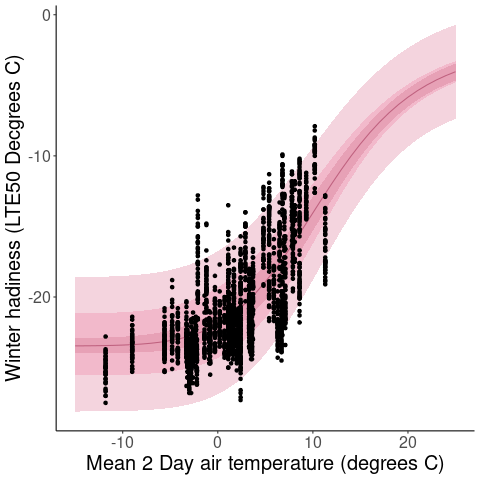
\includegraphics[scale = 0.5]{PredWithReal.png}
  \caption{The points show the winter hardiness data against the corresponding 2 day mean air temperature. The line is the mean model prediction for each temperature, and the darker pink banding is the uncertainty (89\% highest probability index) around this mean prediction. The lighter pink is the uncertainty when the effects of variety and site deviations are considered.}
  \label{fig:predWithReal}
\end{figure}

My model uses all the variety and site data in the same analyses, but checks if there are differences between varieties and sites. Interestingly it finds differences in the maximum hardiness between the varieties. You can see the average maximum winter hardiness of each variety according to my model in Figure \ref{fig:varDs}. Do you agree with these results? I expected Riesling to be more cold hardy and Syrah to be less hardy, and that is what the model found, but I am less familiar with the hardiness of the other varieties. I also looked for differences in the rate of change of hardiness between varieties, but found no difference. Does this surprise you? I know the work coming from Washington (i.e. \cite{Ferguson2014,Ferguson2011}) suggests that there should be different rates of for different varieties. My model also found that different sites had different maximum hardiness values (Figure \ref{fig:siteDs}). Does this figure make sense to you based on how the sites climatically differ from the Penticton weather station? I definitely need the opinion of someone more knowledgeable than I about these sites! \\


\begin{figure}[h]
  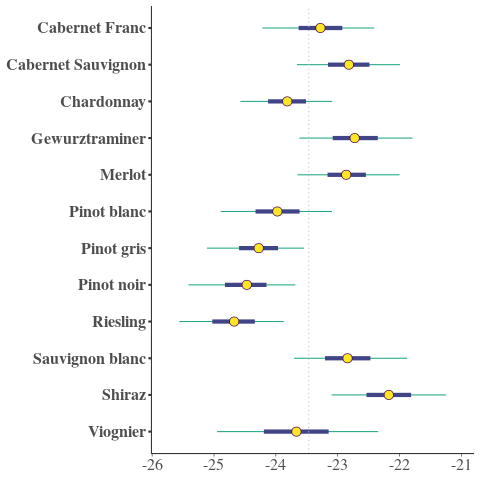
\includegraphics[scale = 0.75]{varDs.png}
  \caption{The variation in maximum hardiness of each variety. The mean value suggested by the model is the circle, and the uncertainty is shown as bars going horizontally away from the circle. The gray dotted line represents the mean maximum hardiness of the overall model.}
  \label{fig:varDs}
\end{figure}

\begin{figure}[h]
  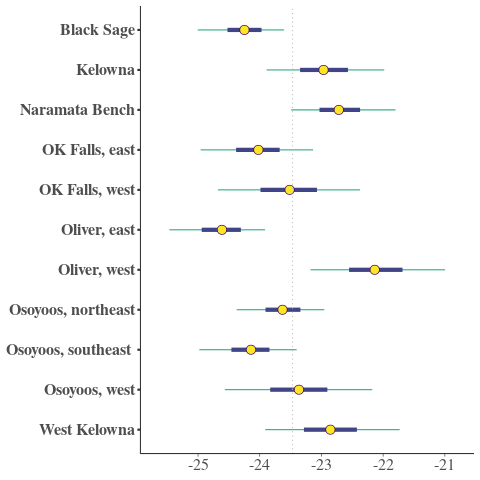
\includegraphics[scale = 0.75]{siteDs.png}
  \caption{The variation in maximum hardiness of each site. The mean value suggested by the model is the circle, and the uncertainty is shown as bars going horizontally away from the circle. The gray dotted line represents the mean maximum hardiness of the overall model.}
  \label{fig:siteDs}
\end{figure}

My plan with this model is not to use it for growers in the Okanagan because your models are much better at that. Instead, I would like to use this model to ask questions about how maximum winegrape cold hardiness has changed over time, and what that means for growers in the Okanagan. I also found that my model did an OK job of predicting Cabernet Sauvignon winter hardiness data from Washington State, so maybe it would be nice to compare what is happening in different regions? I would love to hear if you have some good ideas. \\

\FloatBarrier

\bibliography{/home/faith/Documents/Bibtex/mendeleyStuff/library}

\end{document}

